\documentclass{article}
\usepackage{pgfplots}

\pgfplotsset{compat=1.3}
\usepgfplotslibrary{patchplots}

\begin{document}
\thispagestyle{empty}

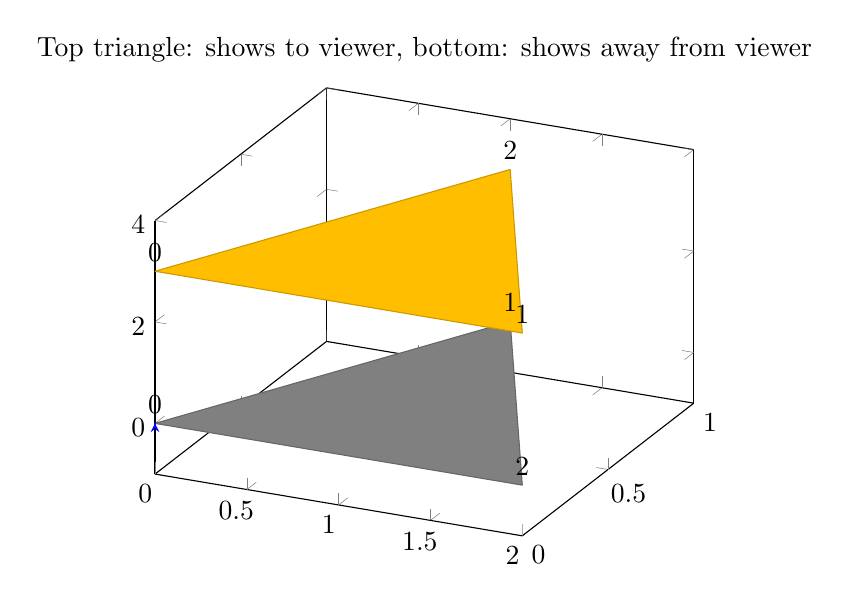
\begin{tikzpicture}
%\tracingmacros=2 \tracingcommands=2
    \begin{axis}[
	zmin=-1,zmax=4,
	title={Top triangle: shows to viewer, bottom: shows away from viewer},
		nodes near coords,point meta=explicit,
		colormap/blackwhite,
		mesh/interior colormap name={hot},
		clip=false,
	]
    \addplot3[patch,table/meta=m]
    table {
        x y z m
        0 0 0 0
        1 1 0 1
        2 0 0 2
% empty lines do not hurt, they are ignored here:

        0 0 3 0
        2 0 3 1
        1 1 3 2
    };
	\draw[-stealth,blue] (axis cs:0,0,0)  \pgfextra{\pgfpathlineto{\pgfpointadd{\pgfplotspointaxisxyz000}{\pgfplotspointviewdir}}};
    \end{axis}
\end{tikzpicture}

\end{document}

